% first example chapter
% @author Jan Robert Rösler 
%
\chapter{Entwurf}
In diesem Kapitel wird der vollständige Entwurf einer Steuerung für ein RC Fahrzeug dargestellt.

Wie im vorangegangenen Kapitel erläutert, entstand die Idee für die Steuerung eines RC-Fahrzeuges mit Neuronalen Netzen im Kontext einer Arbeit der ETH Zürich.
Das dort entworfene DroNet wurde bereits kurz vorgestellt und wird die Basis für die neuronale Steuerung sein. Zunächst sollen darum die technischen Aspekte von DroNet hervorgehoben werden: \\

DroNet ist ein 8-Layer Convolutional Neural Network, das insbesondere aus drei Residual-Blöcken besteht und für den Input eines 200x200 Pixel Bildes in Graustufen zwei Outputs produziert, einmal einen Lenkwinkel aus dem Intervall [-1,1] (hierbei gilt; Werte <0 entsprechen einer Rechtskurve, Werte >0 einer Linkskurve)  und einmal die Kollisionswahrscheinlichkeit in Prozent (als Klassifizierungsproblem in Prozentschritten, nicht kontinuierlich).\\
DroNet hat \num{3.2e5} Parameter und schafft eine Verarbeitungsrate von 20 fps ( Die Drohne, auf der DroNet getestet wurde lieferte Bilder mit 30 Hz).
Wie im vorigen Kapitel bereits erwähnt, wurde DroNet auf einem frei verfügbaren Datensatz trainiert. Im Paper werden dann Ergebnisse mit anderen Netzwerken verglichen, die mit dem selben Datensatz trainiert wurden, um die Performance zu Vergleichen. Ein solcher Vergleich ist für diese Arbeit jedoch nicht sinnvoll, da es um die Anwendung auf ein spezifisches, reales Szenario geht. 

\section{Hardware und Strecke}

Das vom HAW-Team aufgebaute Fahrzeug für den Carolo-Cup (Abbildung~\ref{img:Carolo-Fahrzeug} zeigt die Seitenansicht), besteht, abgesehen von Chassis, Motorelektronik und Servos, im Kern aus einem Intel NUC, auf dem die vollständige Bildverarbeitung und Logik berechnet wird und der Kamera \note{TYP-Kamera}, die die Bilder liefert (montiert an einem Alustab). Die Kontrolle per Fernsteuerung, zum Eingreifen im Fehlerfall und zum Positionieren des Fahrzeugs kommuniziert über Funk direkt mit dem Motorcontroller.\\
Auf dem Intel NUC ist als Betriebssystem Unix eingerichtet.
Eine funktionsfähige Hardware Abstraktion für den Motor und die Steuerungsservos ist vom Carolo-Cup Team bereits entwickelt und steht mir im Weiteren zur Verfügung, diese ist in C++ implementiert.\\

\begin{figure}[h]
	\centering
	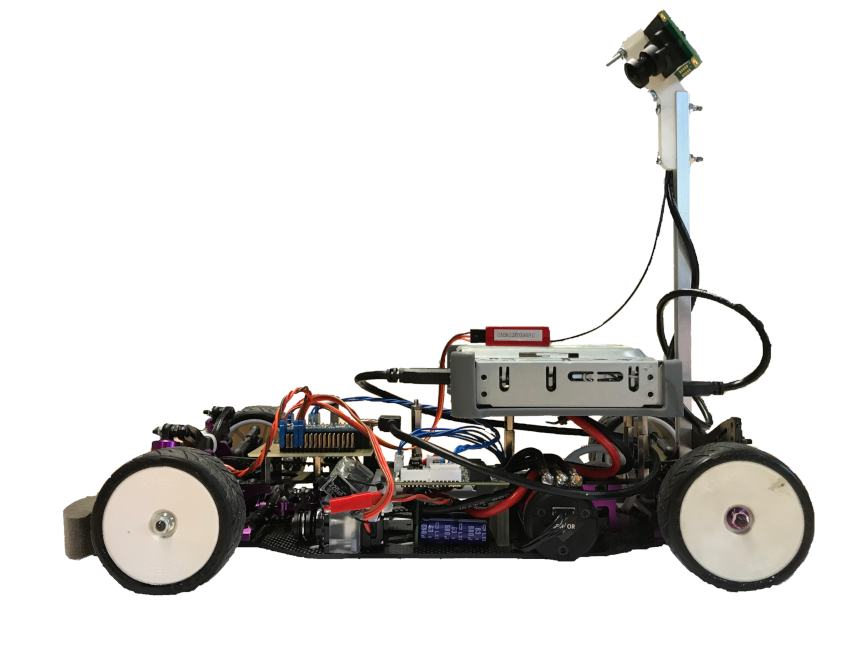
\includegraphics[scale=0.3]{figures/Fahrzeug.png}
	\caption{Das Carolo-Cup Fahrzeug}
	\label{img:Carolo-Fahrzeug}
\end{figure}

Die Teststrecke, die an der HAW zur Verfügung steht, ist ein Rundkurs mit verschiedenen Kurven und einem Kreuzungszenario \note{Collage mit Bildern}. Die Länge der äußeren Fahrbahn beträgt 36,1 Meter, die innere Fahrbahn ist 31,3 Meter lang.\\



\section{Trainingsdaten}



\section{Software und Training}


Adaption auf das Carolo Cup Fahrzeug



Fahren auf der Strecke 

\note{Hervorhaben, welche Teile des DroNet Codes ich weiterverwede. Hard Mining, Auswertungsfunktionen, Architektur}

Änderungen an der Architekrtur des Netzes
Lernarchitekrur (Pipepline)
Steuerungsarchitektur
Bilder mit Steuerdaten (Verarbeitungspipeline) UND VERDOPPELUNG DER DATEN
Fahrzeug (Kamera, Rechner etc.)

Training 
Performance (Rechenzeit) bei prediction auf dem Fahrzeug
Kommunikation zwischen C und pYthon

\note{BILD der STrecke}

\section{Carolo-Cup}
aufgabenstellung beim carolocp
haus eigene strecke etc

\section{Die Strecke}

\section{Das Fahrzeug}
Das Fahrzeug, was von einem Carolo-Cup Team der HAW aufgebaut wurde, wird hier vorgestellt.





Kurzer Blick auf  Self driving car steering angle4 prediction und berkeley (large scale video sets) (vielleicht auchSPÄTER)

